\documentclass{article}
\usepackage{graphicx}
\usepackage{geometry}
\usepackage{float}
\usepackage{fancyhdr}
\usepackage{graphicx}



% Set up page layout
\geometry{a4paper, margin=1in}

% Set up the header
\pagestyle{fancy}
\fancyhf{}
\fancyhead[C]{CMEE Bootcamp Assignment: Sebastian Dohne - 01776389} % Centered header text
\renewcommand{\headrulewidth}{0pt} % Add a horizontal line under the header


\begin{document}

% Centered main section title
\begin{center}
    \section*{Is Florida Getting Warmer?}
\end{center}

% Subsection title
\subsection*{Background and Hypothesis}

The following describes a temporal autocorrelation that was conducted on a dataset containing mean yearly temperature data and their respective years (ranging from 1900-2000) from Key West, Florida to answer the following question:

\begin{itemize}
    \item  Are temperatures of one year significantly correlated with the next year (successive years), across years in a given location?
\end{itemize}

\subsection*{Statistical Analyses and results}
 In R version (version 4.3.3, 2024-02-29), a simple Pearson correlation coefficient was calculated using the cor() function. This resulted in a weak positive correlation coefficient of 0.326 between temperature values in successive years. Temperature values were randomly permuted, and correlation between years was then recalculated 10000 times. A P-value of 4e-04 was generated by calculating what fraction of the correlation coefficients from the random permutations were greater than that from the observed correlation. This confirms our hypothesis that temperature from one year is significantly correlated with temperature from the next year in our dataset. 
\section*{Figure}
\centering
\vspace{2em}

\centering
\begin{figure}[H]
    \centering
    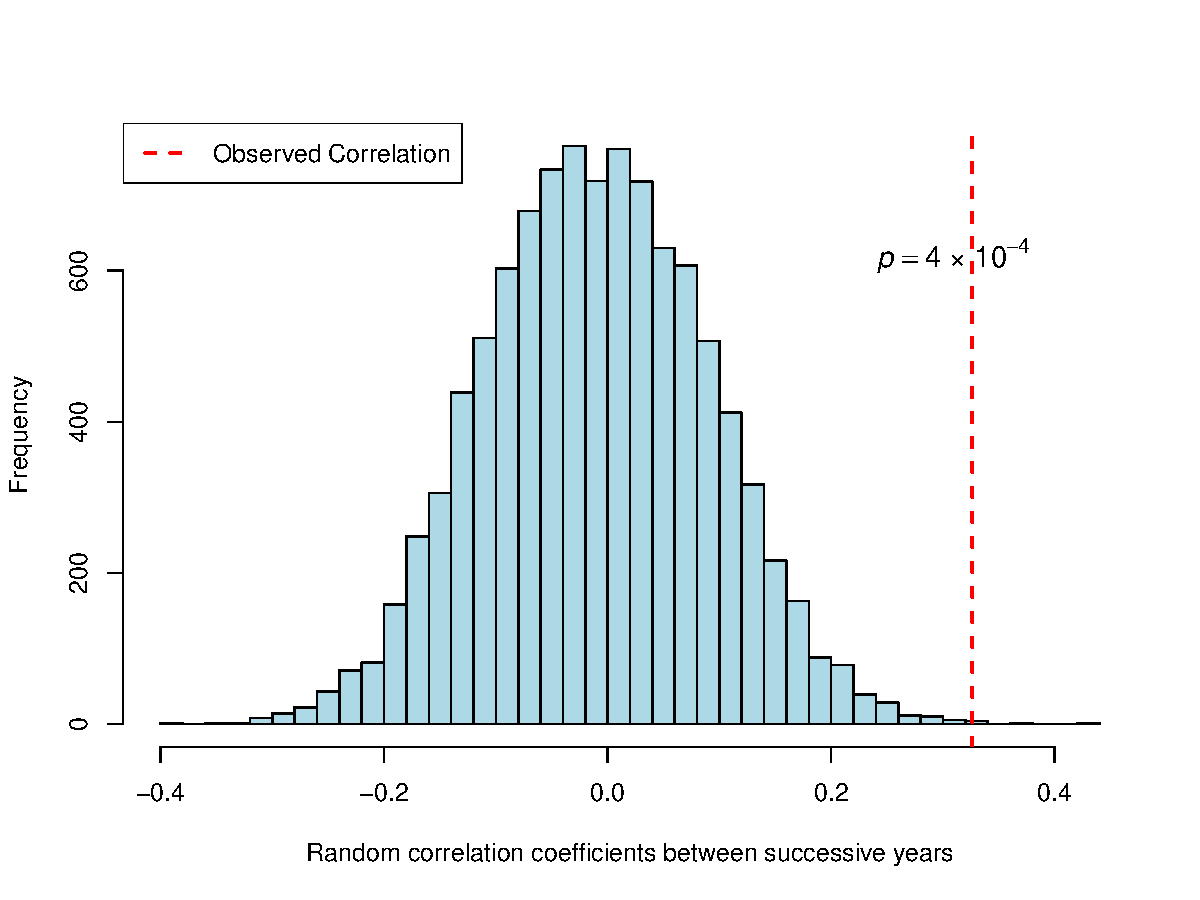
\includegraphics[width=0.9\linewidth]{../data/Coefficients.pdf}
    \vspace{2em}
\caption{Histogram of random permuted correlation coefficients (null distribution) with the observed correlation (red dashed line) highlighted. A small P-value of $4 \times 10^{-4}$ indicates the observed correlation is significantly different from random chance.}
    \label{fig:label2}
\end{figure}

\end{document}
